Dans cette section sont identifiés les points importants qu'il ont été analysés avant de débuter à la conception du jeu. Premièrement, il est expliqué dans la section \ref{sAnaEtatDesLieux} la situation initiale avec un état des lieux afin de préciser où le projet commence, quels sont les composants existants ainsi que leurs interactions. Deuxièmement, les objectifs du projet de recherche et développement (projet R\&D) englobant sont décrits dans la section \ref{sAnaDescriptionObjectifsCTI} avec de premières pistes pour y répondre. Ces dernières étant issues de l'état de l'art où de nouveaux documents. Troisièmement, la section \ref{sAnaContraintes} détaille les contraintes fixées à ce projet (principalement imposées par les composants ou encore le contexte d'utilisation). Finalement, un condensé de tous les points importants à prendre en compte lors de la conception d'un SG de neuroréhabilitation sont listés dans la section \ref{sAnaGameConceptPointsImportant}.
\section{Contexte initial}
	\label{sAnaEtatDesLieux}
	Ce travail de Master précède un projet R\&D. Il fait suite à un autre projet de recherche I2 "SG4R" dont le but était de créer une plateforme de SG. Il est donc important de spécifier ce qui existe actuellement et de définir ce qui doit être fait dans le cadre de ce travail. Voici une liste des composants déjà réalisés ainsi que leur état d'avancement:
	\begin{itemize}
		\item \textbf{LHS --} Le LHS \cite{LHS_website} est le robot de réhabilitation utilisé dans ce projet comme périphérique de réhabilitation. Il est actuellement opérationnel et déjà utilisé par des patients sélectionnés dans le cadre de tests cliniques (utilisant des exercices déjà configurés et validés par le domaine médical et non les SGs). De nombreux algorithmes pour différents types de mouvement y sont présents, mais pas encore celui de la marche qui doit être développé durant le projet R\&D. De plus ample informations sur le périphérique sont présentés dans la section \ref{sAnaContraintes};
		
		\item \textbf{IHM --} L'interface homme machine livrée avec le produit LHS permettant au thérapeute de rentrer les données du patient, de lui configurer et choisir des exercices et également de modifier leurs paramètres en cours d'exécution ou de les interrompre. Une communication entre la IHM et les SGs existe déjà mais très peu de données du SG sont remontées à la IHM;
		
		\item \textbf{Noyau Temps Réel --} Ce noyau garantit de gérer le LHS avec un nombre de millisecondes donné. C'est lui qui remonte les données des capteurs. Une communication entre les SG et l'application temps réel tournant sur ce noyau existe déjà. Cette communication est bidirectionnelle et permet de lire les valeurs des capteurs ou autres entrées prétraitées à l'aide d'algorithmes prenant en compte l'anatomie du patient (\textit{e.g.}, position des pieds) mais également d'écrire des valeurs telles que la difficulté de pédalage (\textit{e.g.}, dut à la pente);
		
		\item \textbf{Communication --} Une API de communication existe mais est très sommaire. Elle a été conçue pour être fonctionnelle avec différents périphériques de réhabilitation;
		
		\item \textbf{Plateforme de SG avec mode \textit{master} et \textit{slave} --} Une plateforme permettant l'accès à quatre SGs fonctionnels, travaillant des exercices différents. Le projet SG4R ne devant pas être lié uniquement au robot LHS, cette plateforme est générique et peut être exécuté d'après deux modes: "\textit{master}", où la plateforme lance l'interface graphique permettant de choisir les jeux; "\textit{slave}", où la plateforme est lancée en arrière-plan et attend que la IHM lui demande de lancer un jeu;
		
		\item \textbf{SGs existants --} Quatre SGs ont été développés à l'aide du moteur de jeu \textit{Unity} \cite{Unity_website} (les scripts ont été écrits en C\# \cite{CSharp_website}) en tant que prototypes afin de les faire valider par le personnel médical. Ces SGs couvraient différents types de mouvement, interactions additionnelles, types de graphisme, types d'immersion et mécaniques de jeu ou d'adhérence. Ces SGs ont impliqué du matériel supplémentaire: un micro ou une souris (améliorée en un bouton tenant mieux en main) et un HMD (casque de réalité virtuelle). Le HMD utilisé est l'\textit{Oculus Rift}, kit de développement 2 (\textit{Oculus Rift DK2}) \cite{OculusDk2_website}.
		Une description plus précise de \textit{Unit}y et de l'\textit{Oculus Rift} est présente dans la section \ref{sAnaContraintes};
		\begin{itemize} 
			\item \textbf{Bike Rehab --} Seul SG en 2D, de style \textit{cartoon}, se passant dans une Italie caricaturée. Le but du jeu est de livrer des pizzas  à vélo en arrivant le plus propre possible (figure \ref{BikeRehab}). Pour avancer (déplacement horizontal à l'écran), il faut pédaler. Les pentes en jeu augmentent la difficulté de pédalage. On peut éviter les obstacles et ramasser des pièces en sautant. Ce saut est effectué soit par contrôle vocal, soit à l'aide d'un bouton dans la main du patient (reproduisant un clic souris). Les pièces amassées (en chemin, en livrant la pizza dans les temps et en recevant un pourboire pour notre propreté) permettent d'acheter des éléments pour personnaliser son avatar et son vélo. Ils changent juste l'aspect graphique et n'influent pas sur le jeu. Six niveaux sont disponibles avec différentes durées, pentes et paysages (ville, campagne, village, vignes et volcan);\medskip
			
			\begin{minipage}{\linewidth}
				\makebox[\linewidth]{
					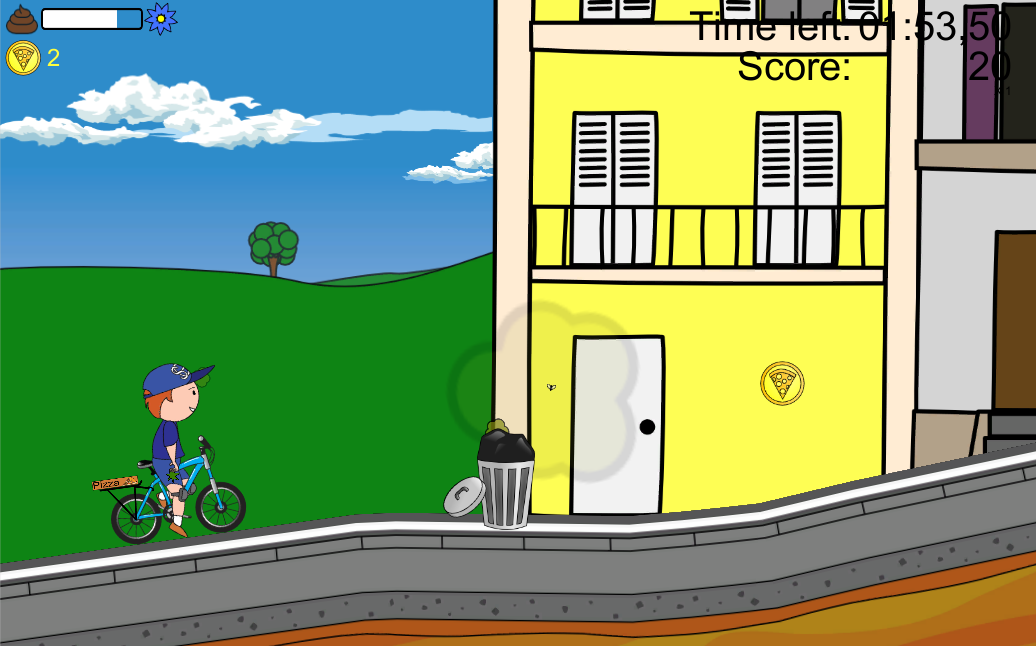
\includegraphics[height=\imgHeightMedium{}]{img/Analyse_BikeRehab2.PNG}}
				\captionof{figure}{Bike Rehab, jeu 2D demandant un exercice de pédalage.}
				\label{BikeRehab}
			\end{minipage}\medskip
						
			\item \textbf{Be The Ball --} Jeu de course où le patient influe sur la vitesse et la direction d'une boule sur un circuit dans un environnement en 3D (figure \ref{BeTheBall}). L'interaction se fait uniquement avec les jambes et s'inspire d'un exercice de \textit{press-leg}. La vitesse est influée par la pression effectuée (le robot reproduisant l'effet d'un ressort) et la direction par la différence de leur position. Un tableau des meilleurs scores par patient est effectué pour chaque niveau et le patient peut voir, durant la partie, une boule fantôme retraçant le parcours effectué par son meilleur score. Quatre niveaux sont disponibles: forêt; île; montagne; désert. Ces niveaux présentent chacun un environnement différent, plusieurs longueur sont représentées et certains tournent plus d'un côté et demande donc plus d'effort d'une jambe spécifique;\medskip
			
			\begin{minipage}{\linewidth}
				\makebox[\linewidth]{
					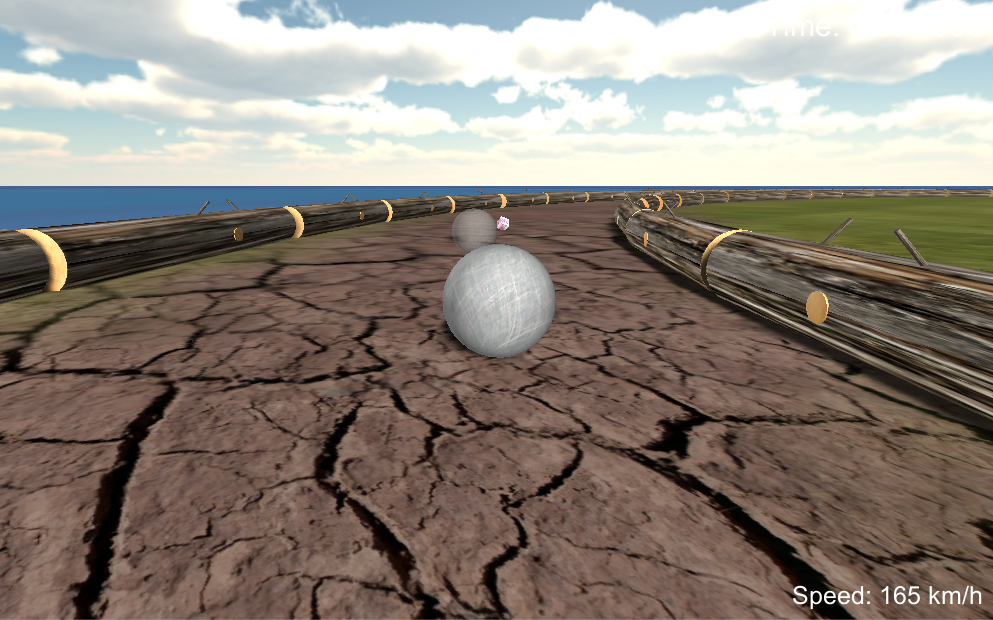
\includegraphics[height=\imgHeightMedium{}]{img/Analyse_BeTheBall2.PNG}}
				\captionof{figure}{BeTheBall, jeu de course demandant un exercice s'inspirant du \textit{press-leg}.}
				\label{BeTheBall}
			\end{minipage}\medskip
			
			\item \textbf{Gate Crossing --} Ce SG se déroule dans l'espace et demande également l'exécution d'un parcours bien définit. Alors que le SG précédent se basait sur une stimulation compétitive, celui-ci essaie de reproduire un environnement relaxant (environnement épuré et musique calme). La vitesse est constante et la direction est donnée par la différence de position entre les jambes (le robot n'applique pas de résistance supplémentaire). Le but étant de passer au centre de portes en faisant le plus de points (figure \ref{GateCrossing}). Contrairement au jeu précédent, on peut sortir du parcours et une redirection automatique est alors effectuée. Ce SG donne la possibilité d'utiliser le HMD mais peut être joué sur un écran également;\medskip
			
			\begin{minipage}{\linewidth}
				\makebox[\linewidth]{
					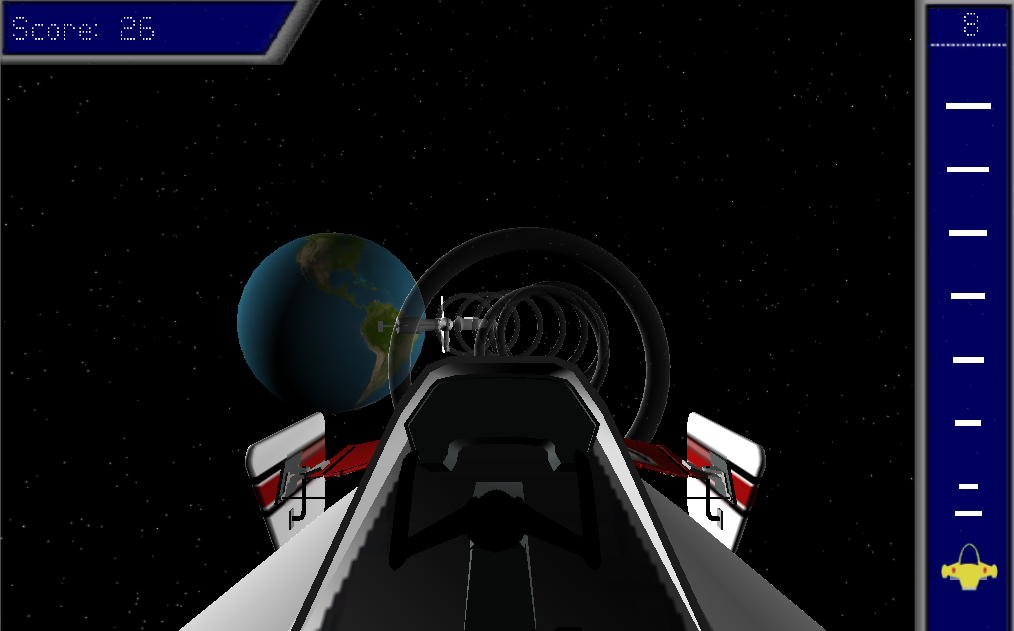
\includegraphics[height=\imgHeightMedium{}]{img/Analyse_GateCrossing2.PNG}}
				\captionof{figure}{Gate Crossing, jeu de précision demandant un exercice s'inspirant du \textit{press-leg}.}
				\label{GateCrossing}
			\end{minipage}\medskip
			
			\item \textbf{Pics Walk --} Ce SG a pour but de travailler la marche et oblige l'utilisation du HMD. Le patient doit donc reproduire un mouvement de marche (qui était simplifié par une ellipse dans un premier temps) avec la particularité de pouvoir réaliser ce mouvement de façon totalement passive. Une interaction supplémentaire était donc nécessaire pour créer une mécanique de jeu. Celle-ci est la prise de photos via contrôle vocal ou bouton (comme le saut de \textit{Bike Rehab}). Le patient peut donc, durant ses différents parcours, prendre certains éléments en photo (figure \ref{PicsWalk}). Quatre parcours dans deux environnements extérieurs différents évoquant la nature sont disponibles. En fonction de l'élément photographié, du cadrage (à l'aide du HMD), de la distance et d'autres facteurs, la photo rapporte certains points. Les photos peuvent être visionnées après une partie.\medskip
			
			\begin{minipage}{\linewidth}
				\makebox[\linewidth]{
					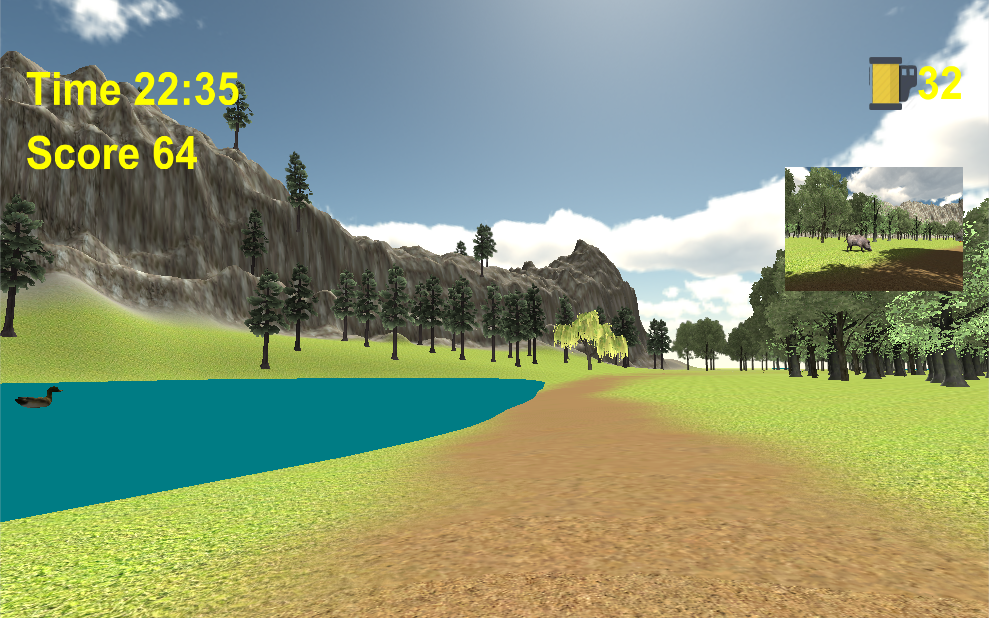
\includegraphics[height=\imgHeightMedium{}]{img/Analyse_PicsWalk2.PNG}}
				\captionof{figure}{Pics Walk, jeu d'exploration et de découverte demandant un exercice de marche.}
				\label{PicsWalk}
			\end{minipage}\medskip
		\end{itemize}		
	\end{itemize}

\section{Identification des objectifs}
	\label{sAnaDescriptionObjectifsCTI}
	Durant le projet R\&D, un seul SG devra être réalisé. Ses objectifs sont cités ci-dessous. À savoir que le SG conçu doit tenir compte de tous les objectifs, mais le délivrable implémenté lors de ce travail de Master ne couvrira qu'une sélection de ces objectifs (sélection effectuée dans la conception, section \ref{sConSelectionObjectifs}).
	
	\begin{itemize}	
		\item \textbf{Interfacés avec le LHS --} Le SG devra être interfacé et opérationnel avec le périphérique de réhabilitation LHS \cite{LHS_website}. Contrairement au projet SG4R, le SG n'aura pas besoin d'être interfaçable avec d'autres périphériques;
		
		\item \textbf{Jeu de marche --} Le SG doit demander au patient d'effectuer un mouvement de marche (qui est guidé ou accompagné par le LHS). Ce mouvement devra être répété longuement durant l'exercice et devra être perturbé le moins possible par d'autres actions. La durée d'un exercice est de 10 à 30 minutes, il faut donc s'assurer que le patient reste attentif et motivé durant toute cette durée;
		
		\item \textbf{Haute immersion --} Trois sens devront être sollicités par des stimuli de l'environnement virtuel. Si un stimulus doit affecter les trois sens, le patient doit les ressentir simultanément. Les sens sont: la vue; l'ouïe; le toucher. Pour la vue, le même HMD (\textit{Oculus Rift DK2} \cite{OculusDk2_website}) doit être utilisé. Il faut prendre garde à éliminer toute saccades du rendu visuel, afin que celui-ci soit fluide et paraisse naturel.
		
		Pour l'ouïe, une recherche d'ambiance sonore et de bruits (tels que les pas sur plusieurs types de terrains) devra être fait de façons approfondie.
		
		Pour le toucher, c'est le retour haptique du LHS qui sera utilisé. Il est souhaitable de simuler plusieurs types de terrains, des pentes ou encore des escaliers. Pour renforcer le toucher, on peut également, si l'on prend l'exemple de \textit{Pics Walk}, donner un appareil photo (ou un objet semblable) dans les mains du patient afin qu'il corresponde mieux à son avatar. Inversement, si le patient doit avoir un périphérique dans les mains, il est souhaitable que son avatar l'aie également;
		
		\item \textbf{Temps réel --} Le contexte d'exécution du SG contient plusieurs composants logiciels et matériels situés sur différents ordinateurs nécessitant de communiquer suite aux interactions de l'utilisateur afin de lui produire un retour (utilisant plusieurs modalités sensorielles). Ce retour doit être perçu comme instantané du point de vue du patient. Il faut donc faire attention à tout temps supplémentaire induit par le système et s'assurer que tous les composants soient synchronisés;
		
		\item \textbf{Représentation du mouvement --} Une représentation du mouvement que le patient effectue (qui est corrigé par le robot) devra être présente dans l'environnement afin d'augmenter le potentiel de la réhabilitation via l'activation des neurones miroirs. Les neurones miroirs sont des neurones qui s'activent à la fois lors de l'exécution d'un mouvement et durant l'observation du même effectué par une autre personne. Cette représentation pourrait donc être les jambes de l'avatar ou d'un autre personnage que l'on doit suivre;
		
		%TODO Peut être parler de ça (mais pas sûr: on ne justifie pas l'objectif qu'on a pas fixer nous...)
		%http://sergibermudez.blogspot.ch/2014/02/virtual-rehabilitation-beyond-gaming.html
		%et
		%"Often video games will include a representation of a player's limb(s) [15, 23, 74]. The use of a graphical representation of the upper extremitites builds on the paradigm of the motor neuron system as a method of augmenting neuroplasticity. Seminal research by neuroscientist Giacomo Rizzolatty prposed that the mirror neuron system activates in both goal-orientated action execution and action observation [101, 102]. Thus, the process of motor learning can occur as a result of watching, as well as physically performing, a movement. By including a virtual representation of a limb, it is hypothesized that the efficacy of a repetition-based exercise can be augmented with motor learning induced by the motor neuron system."
		
		\item \textbf{Niveaux d'appauvrissement et éléments familiers --} Certains patients peinent à interpréter une scène trop riche. %TODO Parler de l'exemple d'une salle de réveil en citant des sources (à faire probablement précédemment dans l'analyse) si documentation trouvée.
		Nos scènes devront pouvoir être affichées avec plusieurs niveaux d'appauvrissement en agissant notamment sur la complexité des éléments (structure, couleurs, animations, etc.) et leur nombre. Ces niveaux doivent prendre le moins de travail possible à être créés (éventuellement envisager des algorithmes les générant). Afin de rassurer le patient, certains éléments familiers (\textit{e.g.}, un cadre avec une photo) devront être présents. Cet aspect n'est pas apparu durant l'état de l'art ni l'analyse car il correspond à une demande directe du médecin collaborant avec le mandant. Demande issue de besoins constatés sur le terrain et n'ayant pas fait, à sa connaissance, l'objet d'études;%TODO: Nommer Rolf ?
		
		\item \textbf{Tests et validations --} Le SG devra être testé et validé par un certain nombre de personnes. Selon Jakob Nielsen une dizaine de personnes suffisent à trouver la quasi-totalité des problèmes. En voulant garantir qu'aucune latence n'est perceptible, 50 volontaires et 15 patients passeront un test. 50 personnes du domaine médical minimum testeront également le système afin de confirmer son objectif médical.
		
	\end{itemize}

\section{Contraintes et choix technologiques}
	\label{sAnaContraintes}
	Dans cette section sont résumés les différentes contraintes matérielles et logicielles concernant le SG à développer.
		\subsection*{Matériel} 
			\begin{itemize}
				\item \textbf{Robot Lambda --} Le robot de réhabilitation à utiliser développé par le mandant de ce projet. Il est composé de deux robots \textit{lambda} (figure \ref{Peripheriques}, image de gauche) un pour chaque jambe \cite{LHS_website}. Ils contiennent des moteurs pouvant assister, apporter de la résistance ou réaliser complètement les mouvements, ainsi que des capteurs de force dont les valeurs sont validées par des capteurs redondants. Les valeurs mesurées, ainsi que d'autres informations prétraitées peuvent être accédées par un logiciel tournant dans le noyau temps réel contrôlant le robot. Les informations prétraitées sont de plus haut niveau, tel que la position du pied, et sont obtenues à l'aide d'algorithmes complexes tenant compte de l'anatomie du patient. Ces informations doivent être utilisées comme une entrée du SG;	
				%TODO: Parler plus précisément des algo.
				
				\item \textbf{Oculus Rift DK2 --} L'utilisation du HMD est une des contraintes du jeu. L'\textit{Oculus Rift}, kit de développement 2 \cite{OculusDk2_website} (figure \ref{Peripheriques}, image de droite) étant actuellement en possession et utilisé par le mandant, il est à utiliser pour le SG. Ce HMD permet une vision stéréoscopique et des capteurs d'orientation permettent de savoir la direction dans laquelle le patient regarde. Des LEDs infrarouges sont également intégrées au casque et, à l'aide d'une caméra (livrée dans le kit de développement), permettent une localisation spatiale de la tête. L'utilisation de cette dernière n'est pas imposée. Elle nécessite une installation supplémentaire du LHS. À utiliser que si cela comporte un réel intérêt;
				
				\item \textbf{Microphone --} Les projets antérieurs se sont servi d'un micro pour certaines interactions à l'aide du contrôle vocal. Ceci vient d'une demande des médecins qui ont identifié le fait que certains patients peuvent présenter des difficultés à effectuer plusieurs actions en même temps. Ceci doit donc être réapprit et il est plus facile et utile de réapprendre à parler en marchant que de se servir d'un joystick. Ce mode d'interaction peut donc être réutilisé mais n'est pas une obligation;
				
				\item \textbf{Joystick --} L'utilisation d'un joystick, d'une manette de jeu ou d'une souris peut être envisageable. Attention cependant à ne pas le rendre obligatoire pour tous les stades de réhabilitation car certains patients n'arriveront pas à s'en servir;
				
				\item \textbf{PC SG --} Pour des raisons de performances et de facilité d'installation, le SG sera exécuté sur un ordinateur différent de celui de l'IHM et du noyau temps réel. Afin de ne pas complexifier la tâche du thérapeute, le PC ne disposera pas de souris ni de clavier et devra lancer le SG dès son démarrage. Le SG devra alors attendre la synchronisation et le signal de départ venant du LHS;
				
				\item \textbf{Casque audio ou haut-parleurs --} L'immersion devant utiliser le sens de l'ouïe, il est nécessaire d'avoir soit un casque audio, soit des haut-parleurs. Le premier ne concerne que le patient et permet une meilleure immersion s'il a une bonne isolation sonore. Si le thérapeute doit cependant communiquer avec le patient, ce dispositif est moins pratique. Des solutions de communication en jeu, via un micro ou des messages prédéfinis pourraient être envisageables. Ces messages font alors complètement parti de la réalité virtuelle où est le patient et peuvent provenir d'un autre personnage. Les haut-parleurs, de leur côté, imposent le son à tous les utilisateurs de la pièce et exposent le patient à des stimuli sonores hors de la réalité virtuelle dans laquelle il est immergé. Le thérapeute peut plus facilement communiquer avec le patient, cependant il y a de fortes chances que la présence du patient dans le jeu s'en voit impactée. \medskip
				
				\begin{minipage}{\linewidth}
					\makebox[\linewidth]{
						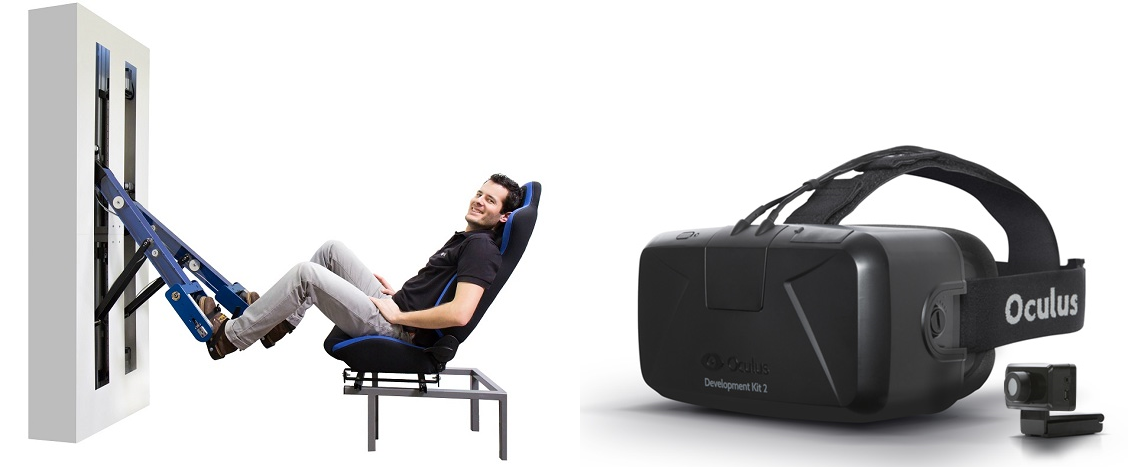
\includegraphics[height=\imgHeightSmall{}]{img/Peripheriques.png}}
					\captionof{figure}{Périphériques utilisés. Dans l'ordre de lecture: LHS; \textit{Oculus Rift}, kit de développement 2.}
					\label{Peripheriques}
				\end{minipage}\medskip	
			\end{itemize}
		\subsection*{Logiciels} 	
			\begin{itemize}
				\item \textbf{Unity \cite{Unity_website} --} Les SGs du projet SG4R ont été réalisés en utilisant le moteur de jeu Unity. Une version tout public gratuite contient l'intégralité du moteur de jeu et permet la création de jeux commercialisables. Ce produit n'est donc pas imposé mais fortement recommandé car il correspond aux attentes du mandant, a fait ses preuves dans les projets antérieurs et permettrait de faciliter la futur maintenance de l'ensemble des SGs. Son utilisation permet également de récupérer bien des éléments déjà développés dans les SGs précédents et ainsi mieux se concentrer sur les nouveaux aspects de ce SG. Pour ces raisons, il a été décidé de continuer à utiliser \textit{Unity} en écrivant les scripts en\textit{ C\#} \cite{CSharp_website};
				% Ayant participé aux projets antérieurs ainsi qu'au cours \textit{Game Technologies} du MSE qui a donné une formation sur ce moteur également, la prise en main sera facilité. Unity a été choisit (avec l'écriture des script en C\#).
				
				\item \textbf{Objectis Communication Foundation (Ocf) \cite{OcfClient_website} --} Cette technologie développée par Objectis \cite{Objectis_website} permet la simplification de la communication entre deux applications. Elle est imposée par le LHS car utilisée pour la communication entre les différents composants. Elle est donc à utiliser pour récupérer ou envoyer des données au LHS. Elle est basée sur une architecture client/serveur. Le serveur met à disposition une série d'objets que le client peut venir lire ou écrire de manière transparente.
				
				Dans le projet précédent, l'échange d'informations a été réalisé avec le protocole UDP et l'API d'Ocf \cite{OcfClient_website}. Cette dernière est écrite en \textit{C\#} \cite{CSharp_website} et utilise les types dynamiques présents uniquement depuis le \textit{framework} ".NET 4.0" \cite{DotNetFramework_website}.
				\textit{Unity} quant à lui utilise la version 2.0 de ce \textit{framework}, ce qui rend l'utilisation directe d'Ocf impossible depuis \textit{Unity}. La communication a alors été réalisée (pour le projet SG4R) via un programme supplémentaire. Celui-ci communiquant avec le jeu via mémoire partagée. L'utilisation d'Ocf est donc obligatoire et la mémoire partagée est fortement recommandée.
			\end{itemize}		
		
		\subsection*{Contextuels}
			Le patient jouera aux SGs à l'hôpital (ou en clinique) car le LHS ne prévoit pas (pour le moment) une utilisation à domicile. Cela implique quelques contraintes contextuelles qui influent sur la conception du SG.
			\begin{itemize}
				\item \textbf{Fréquence des sessions --} La fréquence des sessions de réhabilitation est de une à cinq par semaine. Elles durent une heure, mais il ne faut compter que 10 à 15 minutes de SG. De plus, le SG ne sera pas obligatoirement utilisé à chaque session. On peut donc mettre en place un mécanisme de récompense (et non de punition) hebdomadaire;
				\item \textbf{Présence du thérapeute --} Le thérapeute est présent tout au long de l'exercice. C'est lui qui doit choisir l'exercice ainsi que ses paramètres. Il doit pouvoir modifier la difficulté si besoin. Le LHS avec son IHM possède déjà une interface convenant aux thérapeutes pour régler et agir sur un exercice. Si le SG doit contenir des réglages (paramètres de difficulté, choix du niveau, etc.) et des retours supplémentaires pour les thérapeutes (\textit{e.g.}, score "héminégligence"), ils doivent être disponibles via cette interface. Ces interfaces devront être le plus simple d'utilisation et d'interprétation possible.
			\end{itemize}		
	
\section{Éléments pour la conception d'un SG de neuroréhabilitation}
	\label{sAnaGameConceptPointsImportant}
	Dans cette section sont détaillés tous les éléments à prendre en compte pour la conception d'un jeu d'après la documentation trouvée. L'accent est mis sur les implications et concrétisations des objectifs listés précédemment.
	\begin{itemize}
		\item \textbf{Présence et immersion --} D'après Witmer et Singer REF, quatre facteurs clés détermine la présence \cite{Witmer_MeasuringPresence}:
		\begin{enumerate}
			\item \textbf{Facteur sensoriel --} La figure \ref{5Senses} représente la qualité de l'immersion et la difficulté de rendu d'une réalité virtuelle pour chaque sens ajouté (somme cumulée). On remarque que dès l'ajout du touché, on obtient une immersion presque totale.
			
			\begin{minipage}{\linewidth}
				\makebox[\linewidth]{
					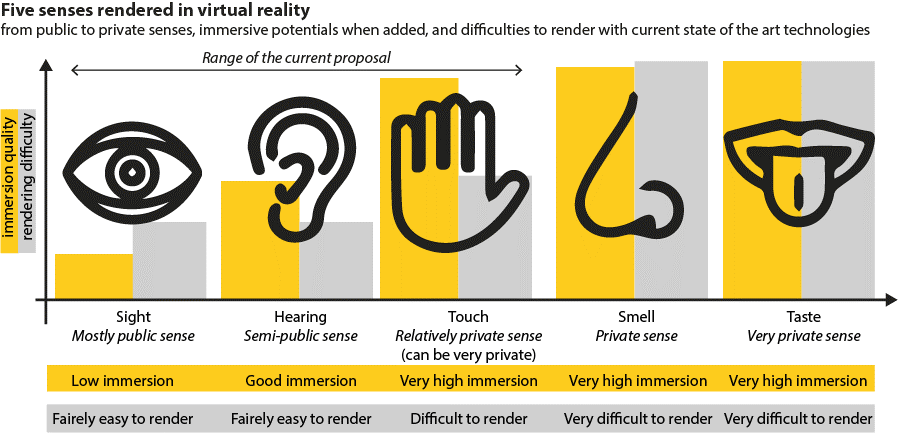
\includegraphics[height=\imgHeightMedium{}]{img/Analyse_5SensesInVR.png}}
				\captionof{figure}{Difficulté d'implémentation et renforcement de la présence pour les cinq sens en réalité virtuelle.}
				\label{5Senses}
			\end{minipage}\medskip
			
			À noter que le facteur sensoriel ne dépend pas uniquement de la présence de stimuli pour les sens souhaités mais également de leur qualité.
			
			Pour ce projet, les sens ciblés sont la vue, l'ouïe et le toucher. La vue est stimulée à l'aide du HMD. L'ouïe à l'aide d'un casque audio ou d'haut-parleurs. Le touché via le retour haptique du robot qui devra donner aux jambes l'impression réelle de l'action qui est en train d'être effectuée (\textit{e.g.}, type de terrain, pente, escalier);
			
			\item \textbf{Facteur de contrôle --} Plus le patient a un sentiment de contrôle, plus sa présence sera renforcée. Ce sentiment de contrôle est basé sur les interactions que le joueur peut avoir avec son environnement afin qu'il se sente acteur et non spectateur.	
			En plus des interactions, il faut que le \textit{game flow} soit bon. Ce dernier étant bon si l'équilibre entre le challenge demandé et les capacités de la personne est respecté (plus de détails sur sa définition et ses implications décrit au point suivant). Trop de challenge induirait de l'anxiété et trop peu de l'ennui. Si ce \textit{game flow} est bon, le patient aura alors un sentiment de contrôle et sa présence sera renforcée;
			
			\item \textbf{Facteur de distraction --} Les distractions liées à l'environnement réel du joueur doivent être réduites au minimum. En utilisant un HMD et un casque audio avec une forte isolation, on peut ainsi garantir que tous les stimuli visuels et sonores viennent de l'environnement virtuel et non de l'environnement réel. Attention, cela peut, dans notre cas, être contraire au besoin qu'a le thérapeute de communiquer avec le patient. Pour maximiser la présence du joueur mais tout de même permettre au thérapeute de communiquer avec le patient, il est possible de placer un autre agent dans l'environnement qui donnerait les instructions que le thérapeute dicte (au micro ou à l'aide de messages préenregistrés).			
			L'interface du jeu et les différents retours d'informations ne doivent pas non plus distraire le joueur;
			
			\item \textbf{Facteur de réalisme --} Le réalisme ne comprend pas uniquement de beaux graphismes, mais une cohérence entre les différents éléments de la scène (\textit{e.g.}, source de lumière et ombre). Chacune de ces incohérences peut alors diminuer la présence de l'utilisateur. Il est important de se souvenir de ce point durant le développement, cependant, la plupart de ces détails seront réglés par le moteur de jeu lui-même. À nous, par contre, de trouver des éléments étant cohérents placés ensemble dans la même scène (style graphique).
		\end{enumerate}
		
		\item \textbf{Game flow - expérience optimale --} Le \textit{game flow} est le ressentit de l'utilisateur sur le challenge que le jeu demande. Le sentiment d'avoir le contrôle sur le jeu \cite{Salen_RulesOfPlay}. Il est bon si l'équilibre entre le challenge demandé et les capacités de la personne est respecté. Trop de challenge induirait de l'anxiété et trop peu de l'ennui. Le niveau optimal ce situe lorsque la tâche est difficile mais faisable \cite{Green_ExercisingBrain}. C'est dans cet équilibre que le joueur aura une expérience optimale du jeu.
		\\
		
		Une des techniques utilisée pour maintenir un bon \textit{game flow} est l'ajustement automatique de la difficulté \cite{Alankus_TowardsCustomizableGames, Cameirao_RehabilitationGamingSystem, Burke_DesigningEngagingPlayableGames4Rehab}. Le challenge augmente plus le joueur réussi et diminue quand il échoue (figure \ref{DifficultyAdjustment}). Une évaluation faîte par Burke et al. \cite{Burke_DesigningEngagingPlayableGames4Rehab} a montré un intérêt des joueurs à ce système d'équilibrage, même pour des personnes saines (80\% ont remarqué cet ajustement et l'ont apprécié). Attention cependant à ce que cet équilibrage ne soit pas trop brusque et que la difficulté n'augmente pas trop rapidement dès que le patient réussi. L'analyse de l'augmentation et de la diminution de ces facteurs permet également une étude plus approfondie des capacités de l'utilisateur au long d'une session d'exercices. Il est possible de proposer des niveaux de difficulté (facile, intermédiaire, expert) contenant tous un ajustement automatique de la difficulté mais variant le seuil de réussite ou d'échec avant de modifier les paramètres. Si la difficulté ne réside pas dans l'exécution du mouvement de réhabilitation (comme les SGs "Bike Rehab" et "Pics Walk" du projet SG4R), il est envisageable de laisser l'utilisateur la régler. En lui montrant l'influence de chaque paramètre sur la récompense finale, il pourra alors essayer des réglages plus dur pour gagner plus. L'utilisateur fixant son propre but a alors plus de contrôle et peut augmenter sa motivation \cite{Nagle_DifferentDifficultyAdaptation}.
		
		\begin{minipage}{\linewidth}
			\makebox[\linewidth]{
				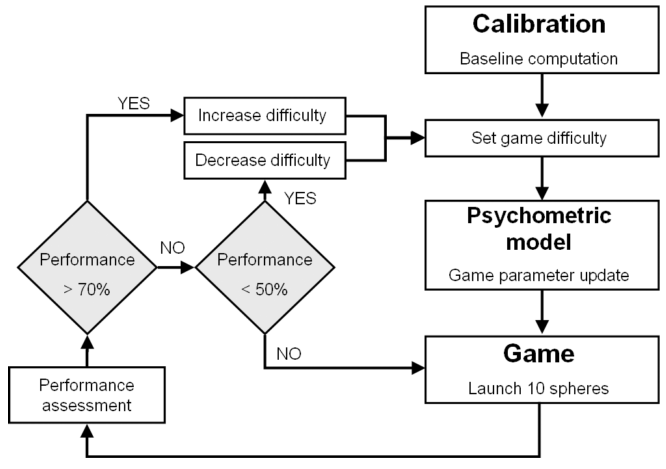
\includegraphics[height=\imgHeightMedium{}]{img/Analyse_Cameirao_DifficultyAdjustment.PNG}}
			\captionof{figure}{Diagramme d'ajustement automatique proposé par Cameirão et al. \cite{Cameirao_RehabilitationGamingSystem}.}
			\label{DifficultyAdjustment}
		\end{minipage}\medskip
		
		Les paramètres souvent utilisés dans les SGs pour la réhabilitation sont: la taille, la vitesse et le lieu des différents objectifs. Ces paramètres, avant de s'ajouter automatiquement, doivent être initialisés manuellement ou par une calibration. Dans tous les cas, le thérapeute doit pouvoir modifier ces paramètres. En modifiant ces paramètres il peut également être possible de travailler différents aspects d'un objectif tels que la vitesse ou la précision \cite{Alankus_TowardsCustomizableGames}.
		
		Dans un jeu habituel, la gestion de la difficulté est souvent en lien avec le nombre d'échec que va subir le joueur. Dans un SG de réhabilitation, l'échec doit être traité avec précaution. Trop d'échec pourrait rapidement être lié à une perte d'engagement car le patient l'associe directement à ses propres capacités motrices et physiques. C'est pourquoi Burke et al. \cite{Burke_DesigningEngagingPlayableGames4Rehab} recommandent d'aborder cet échec de façon encourageante (\textit{e.g.}, ne pas dire "Vous êtes mort. Réessayer ?" mais plutôt "Félicitations, vous avez obtenu 150 points.");
		
		\item \textbf{Environnement virtuel --} Une étude a été menée sur 14 participants pour savoir si un environnement virtuel naturel induisait plus de relaxation et moins d'anxiété qu'un environnement virtuel urbain. Cette étude se fit en deux étapes. La première montrait simplement l'environnement sur un écran. Le résultat montra une faible préférence pour l'environnement naturel mais pas de manière significative. La deuxième étude montra qu'en ajoutant une ambiance sonore, l'anxiété augmenta et la relaxation diminua dans l'environnement urbain alors que l'inverse a été observé dans l'environnement naturel \cite{VARSG4HC1}.
		Un dernier aspect notable est que, d'après Alankus et al. \cite{Alankus_TowardsCustomizableGames}, si l'environnement contient des personnages non joueur, il serait souhaitable de pouvoir interagir avec eux;	
		
		\item \textbf{Temps réel --} Afin de garantir que le SG puisse être considéré comme une application temps réel, on doit s'assurer que les différents retours utilisateur soit générés dans un maximum de temps donné, ne provoquant ainsi pas de perception de latence et n'augmentant pas le taux d'erreur de l'utilisateur. Une étude \cite{Jay_RT_ModelingEffectsDelayedHaptic} a montré que s'il fallait 50 ms de latence (temps entre l'interaction et le retour d'information) visuelle pour qu'une personne la remarque (pouvant provoquer des \textit{Breaks In Presence}), il en faut 25 de moins pour l'haptique. En effet, à plus de 25 ms, la latence n'est pas forcément perceptible, cependant le taux d'erreur de l'action augmente. Pour garantir la cohérence lors de la réhabilitation, il faut donc que l'haptique et les autres modalités soient à moins de 25 ms de latence. Autrement dit, chaque action que l'utilisateur effectue doit avoir déclenché des retours dans les modalités souhaitées en moins de 25 ms;
		
		\item \textbf{Progression --} D'après Dennis W. Fell  \cite{Fell_ProgressingTherapeuticInvervention}, la progression est un élément clé de l'apprentissage moteur. Elle doit se faire durant une session mais également sur l'ensemble de la réhabilitation. Cette progression peut se concrétiser avec l'augmentation du niveau de difficulté. Cette progression à court et long terme doit également être visible par le patient afin d'augmenter son engagement \cite{Burke_DesigningEngagingPlayableGames4Rehab};
		
		%TODO: Parler des courbes d'évolution de difficulté
		
		\item \textbf{Principe de l'apprentissage moteur --} Pour qu'un SG soit efficace dans le cadre d'une réhabilitation, il doit comprendre des instructions, des \textit{feedbacks} et un agenda d'entraînements appropriés \cite{SGVW_EducationProfDevHealthCare}. Il doit également présenter des informations individualisées pour différents types d'individus et différents stades d'apprentissage. Le livre donne également quatre points pour un apprentissage qui se fait de façon transparente:
		\begin{itemize}
			\item \textbf{Adaptativité --} Donner des astuces ou retour d'informations adaptables au patient, ou encore lui adapter son environnement;
			\item \textbf{Adaptation et personnalisation --} Constitutionnelle, qui s'adapte aux dimensions d'une personne et autres contraintes physiques. D'après les préférences et capacités cognitives de l'utilisateur. Physiologique, qui agit en cours de partie, d'après les capacités physiques actuelles du patient mais également sur le long terme, entre plusieurs sessions;
			\item \textbf{\textit{Game mastering} --} Le jeu ne peut pas tout savoir. Il faut quelqu'un qui connaisse bien le jeu et le but pour pouvoir évaluer au mieux les performances et donner de bons retours (dans notre cas: les thérapeutes);
			\item \textbf{Reconnaissance d'activité et détection d'erreur --} Reconnaître le mouvement que le patient est en train d'effectuer et pouvoir mesurer un degré de réussite ou d'échec.
		\end{itemize}
		
		\item \textbf{Addiction --} Comme dans la plupart des jeux actuels, l'identification et l'achèvement d'objectifs permet de stimuler la compétitivité d'un joueur et de maintenir son engagement.
		%TODO: Approffondir après avoir lu le livre.
		%"Modern video games aim to engage the user in extended periods of play whereby large volumes of repetitive button presses are required to complete on-screen objectives. The mechanisms which mediate the upkeep of this behavior are a complex and diverging multidisciplinary study in itself [105].
		
		Les récompenses sont un moyen de maintenir l'engagement du joueur. Cependant si celles-ci sont trop régulières elles finissent par le lasser. Induire un aléa dans la distribution de récompenses ou la baser sur des paramètres variables permet de maintenir une plus grande motivation. Cette attribution des récompenses peut être basée sur des préférences utilisateur, certains nécessitant plus d'encouragements que d'autres \cite{Nagle_PlayerCenteredRewardScheduling};
		
		\item \textbf{Feedback --} D'après Dennis W. Fell \cite{Fell_ProgressingTherapeuticInvervention} les feedback sont un élément clé de l'apprentissage moteur et doivent être nombreux au début afin que le patient puisse se corriger et progresser. Cependant, plus le patient progresse, plus les feedbacks doivent diminuer laissant ainsi de l'autonomie au patient;
		%TODO: En parlé quand les full-texte sont reçu (demande envoyé sur la plateforme de recherche).
		%"Feedback is the mediator between the system and player, and is known to be an important motivator for motor learning [2]." 
		
		\item \textbf{Interactions --} Alankus et al. ont publié un article \cite{Alankus_TowardsCustomizableGames} partageant leurs expériences acquises durant le développement de SGs pour patient atteint d'un AVC. Voici de leurs recommandations, celles pertinentes dans notre cas pour les interactions.
			
		Premièrement, pour permettre aux patients présentant différents niveaux de réhabilitation de jouer au SG, il est souhaitable de pouvoir utiliser plusieurs périphériques d'entrée.	Deuxièmement, le public cible pouvant présenter des troubles cognitifs et n'étant pas obligatoirement habitué aux jeux vidéo, les interactions doivent être les plus naturelles possibles. Pour finir, il est tout de même souhaitable de donner la possibilité de réaliser des interactions complexes demandant la coordination de plusieurs actions pour progresser dans la réhabilitation des tâches de tous les jours. Ainsi, plusieurs interactions évoluant au cours de la réhabilitation seraient souhaitables. 
		
		Si l'interaction que l'utilisateur réalise est liée à un mouvement physique, il existe également des lois décrivant la vitesse attendue d'après certains facteurs. La loi de Fitts semble adéquate pour régler la difficulté via la vitesse pour un jeu de réhabilitation du bras. \cite{Zimmerli_ValidationBalanceDifficulty}.
	\end{itemize}	
